\documentclass[10pt, a4paper]{article}
\usepackage[ngerman]{babel}
\usepackage[utf8]{inputenc}
\usepackage[T1]{fontenc}
\usepackage{color}
\usepackage{hyperref}
\usepackage{comment}
\usepackage{enumitem}
\usepackage[backend=biber,style=alphabetic,]{biblatex}
\usepackage{graphicx}
\usepackage{wrapfig}
\usepackage{caption}
\DeclareCaptionFormat{citation}{%
   \ifx\captioncitation\relax\relax\else
     \captioncitation\par
   \fi
   #1#2#3\par}
\newcommand*\setcaptioncitation[1]{\def\captioncitation{\textit{Source:}~#1}}
\let\captioncitation\relax
\captionsetup{format=citation,justification=centering}
\graphicspath{ {./images/} }

\addbibresource{literature.bib}

\title{Projektbreicht Smart Music Player}
\author{Anton Bracke\\Jan Eberlein\\Tom Calvin Haak\\Julian Hahn\\Nick Loewecke}

\begin{document}
\maketitle
\newpage
\tableofcontents
\newpage

\section{Einleitung}
Ein zentraler Teil des Studiengangs \glqq Informationstechnologien\grqq{} ist es, Softwareentwicklung in Teams und Kommunikation mit Kund:innen zu erlernen. \cite{Qualifikationsziele_Informationstechnologie}
Dies passiert vor allem im Modul \glqq Projekt Informatik (PROI)\grqq{}.
In diesem arbeiten Studierende ein Semester lang in kleinen Gruppen an verschiedenen Projekten.
Diese bilden häufig reale Sachverhalte der Softwareentwicklung ab und werden meist von Firmenpartner:innen aus der Wirtschaft gestellt.
Die Teams wählen ein oder mehrere Projekte, die sie gerne bearbeiten würden, und stellen sich mit einer Kurzbewerbung bei den entsprechenden Firmen vor.
Welche Teams die jeweiligen Projekte bearbeiten, entscheiden die Firmen selbst.
\\
Dieser Bericht beschreibt das Projekt und dessen Verlauf, dass das Autoren-Team für die macio GmbH aus Kiel bearbeitete.

\subsection{Unternehmen}
\colorbox{red}{TODO:}was macht macio aus
\subsection{Projektidee}
Im Rahmen des Projekt Informatik möchte Macio ihr Portfolio im IoT-Bereich erweitern, sowie ihren Empfangsraum im Standort Kiel verschönern.
Hierfür soll eine smarte Spielzeug-Box gebaut werden.
Smarte Spielzeuge gibt es im kommerziellen Bereich viele, daher soll dieses Projekt eine Open-Source-Alternative schaffen.\\
Genauer handelt es sich um eine Musik-Box, die NFC-Chips lesen und Spotify Connect unterstützen soll.
Auf die Box können dann Spielzeuge (z.B. in Form von kleinen Figuren) mit integrierten NFC-Chips gestellt werden, um spezifische Musik abspielen zu lassen.
Die Musik wird von Spotify-Connect über eine bereits bestehende Musik-Anlage abgespielt.
Falls es im Rahmen des Projektes möglich ist, sollen die Nutzer in der Lage sein, zwischen verschiedenen Musikanbietern zu wechseln.
NFC-Chips und die zugehörige Musik sollen über ein Web-basierte Benutzeroberfläche konfiguriert werden können.
Diese Benutzeroberfläche soll von der Box ausgeliefert und primär für Smartphone-Bedienung gestaltet werden.
Da es sich um ein Open Source Projekt mit entsprechender Lizenz handelt, muss auch eine aussagekräftige, öffentliche Dokumentation verfasst werden.
Macio stellt die benötigte Hardware zur Verfügung und unterstützt bei technischen Fragen.

\subsubsection{Minimal Requirements}
\begin{enumerate}
  \item NFC-Tags lesen, schreiben und entschlüsseln
  \item Mit Spotify Connect verbinden und arbeiten
  \item Responsive UI konzeptionieren und umsetzen
  \item Aussagekräftige Dokumentation mit Benutzerhandbuch
\end{enumerate}
\subsubsection{Stretch Goals}
\begin{enumerate}
  \item Sound Wiedergabe auf der Box selbst
  \item Unterstützung anderer Musikdienste / Plugin-Subsystem
  \item 3D-Modellierung und Print einer passenden Box
  \item Cloud-Anbindung der Box, Auslieferung des UI aus der Cloud
\end{enumerate}

\section{Projektplanung}

\subsection{Projekt Management}
Am Anfang des Projekt entschied sich das Team in Abstimmung mit macio für eine agile Projektorganisation.
Diese Richtung des Projektmanagements zeichnet sich vor allem durch fortlaufende Produktentwicklung, kontinuierliches Feedback, kooperatives Arbeiten und Reaktionsfähigkeit bei Anforderungsänderungen aus.
Diese Entscheidung geschah aus mehreren Gründen.
Zum einen haben agile Methoden kein festes Endprodukt als Ziel, wie es beispielsweise bei klassischer Softwareentwicklung (Wasserfallmodell, V-Model, etc) der Fall ist.
Solch ein festes Ende würde der geforderten Veröffentlichung als Open-Source-Projekt nicht gerecht werden, da solche per Definition erweiterbar sind.
Des weiteren haben agile Entwicklungsprozesse vergleichsweise kürzere Veröffentlichungszyklen.
Dies ermöglichte dem Team ein funktionierendes Produkt innerhalb des recht knappen Zeitrahmens eines Semesters\footnote{Dieses Semester wahr aufgrund besonderer CoViD19-bedingten Auflagen einige Wochen kürzer als ein typisches.} zu erstellen.
\\
Entsprechend der Entscheidung zu agiler Entwicklung wurde zu Beginn des Projekt keine feste Planung des Projektverlaufs aufgestellt.
Stattdessen entwickelte das Team eine Methodik um iterativ im Projekt zu arbeiten.
Orientiert wurde sich hierbei an der Methode Scrum.
Aus dieser wurden vor allem die Einteilung in Projektiterationen fester Länge (Sprints) und die zugehörigen wiederkehrenden Meetings übernommen.
Diese Sprint waren im allgemeinen zwei Wochen\footnote{Abgewichen wurde von dieser Länge nur zum Jahresende, um die Feiertage unterzubringen.} lang.
Die Rollen der Teammitglieder in Scrum wurde nicht adaptiert, da sich im Team für eine Gleichverteilung der Aufgaben entschieden wurde.

\subsubsection{Vor den Sprints}
Den Anfang eines jeden Sprints stellte das Sprint-Planing dar.
Im diesem stellte das Team eine Vision für die Sprintiteration auf.
Diese wurde gemeinsam mit dem Kunden abgesprochen und gegebenenfalls abgeändert.
Im Anschluss wurde die Produktvision vom Team in technisch orientierte Arbeitspakete aufgeteilt.
Dies geschah anhand des geschätzten zeitlichen Arbeitsaufwands der einzelnen Änderungen.
Falls sich hierbei gegebenenfalls herausstellte, dass einzelne Arbeitspakete nicht umsetzbar oder zu aufwändig waren, wurde die Produktvision entsprechend angepasst.


\subsubsection{Arbeit in den Sprints}
Während der Sprints wurde die Produktvision aus den Sprint-Planings implementiert.
Alle Mitglieder des Team waren an dieser Arbeit beteiligt.
Die einzelnen Arbeitspakete wurden entweder alleine, in Paaren oder selten auch in Gruppen bearbeitet.
Dies wurde anhand der Anforderung und des Aufwands der jeweiligen Arbeitspakete entschieden.
Auch das spezifische Fachwissen der beteiligten Personen hatte einen Einfluss auf die Aufteilung.
In jedem Fall wurden die Pakete erst bei Arbeitsbeginn und nur von den bearbeitenden Mitgliedern selbst zugewiesen.
\\
Nach Bearbeitung eines Paketes wurden die vollzogenen Änderungen durch Code Reviews von mindestens zwei anderen Entwicklern geprüft.
Nur wenn diese erfolgreich waren, wurde der entsprechende Code ins Produktinkrement übernommen.
Dieses Verfahren wurde angesetzt, um sowohl Flexibilität von Arbeitszeiten zu ermöglichen, als auch um die gewünschte Produktqualität sichherzustellen.
Verschiedene Arbeitszeiten waren notwendig, da alle Teammitglieder verschiedene parallele Veranstaltungen besuchten und anderen beruflichen Tätigkeiten nachgingen.
So waren keine langfristigen synchronen Arbeitszeiten aller Mitglieder möglich.
Die freie Verteilung von Paketen ermöglichte auch, dass Mitglieder in persönlich bevorzugten Themengebieten arbeiten konnten.
Dies half die Motivation des Teams am Projekt hochzuhalten.
\\
Um sich während der Sprints abzustimmen und um Arbeitsfortschritte abzugleichen, trafen sich die Teammitglieder drei Mal pro Woche.
Dies geschah immer montags, mittwochs und freitags.
Bei Bedarf wurde auch von dieser Taktung abgewichen.
In Aufbau und Zweck orientierten sich diese regelmäßigen Meetings an den \glqq Daily Standups\grqq{} der Scrum-Methode.
Während den Meetings stellte jedes Teammitglied kurz vor was es seit dem letzten Standup am Projekt bearbeitet hatte, welche Probleme dabei aufgetreten waren und was bei der Arbeit gelernt wurde.
Auch welche Themen jedes Mitglied bis zum nächsten Standup bearbeiten wollte, wurde besprochen.
Nach diesen Kurzvorstellungen wurden einzelne besonders interessante und wichtige Punkte der Arbeit oder gelöste Probleme im Detail besprochen.
So konnte das Team auf den gleichen Wissensstand kommen und gemeinsam Entscheidungen treffen.

\subsubsection{Am Ende der Sprints}
Nach jedem Sprint wurde das Ergebnis bzw. das Produktinkrement dem Kunden und der Projektbetreuung vorgestellt.
Hier wurde meist auch zusammen mit macio das Ausmaß des nächsten Produktinkrements besprochen.
Die resultierenden Wünsche und Rückmeldungen wurden mit ins Backlog und die folgenden Besprechungen mitgenommen.
Im Anschluss fand immer eine Retrospektive statt.
In dieser besprach das Team die eigene Zusammenarbeit und den gemeinsamen Umgang.
Hierfür stellten sich alle Teammitglieder für sich folgende Fragen für die Arbeit am entsprechenden Sprint:
\begin{itemize}[noitemsep,topsep=0pt,parsep=0pt,partopsep=0pt]
  \item Was lief gut?
  \item Was lief schlecht?
  \item Was habe ich neu gelernt?
  \item Was können wir in Zukunft besser machen?
\end{itemize}
Die jeweiligen Antworten wurden zusammengetragen und im Team gemeinsam reflektiert.
Das Feedback in diesem Kontext war konstruktiv und fair aber auch ehrlich.
Die daraus entstandenen Erkenntnisse und Verbesserungsvorschläge wurden genutzt um das Teamwork und die Arbeit im folgenden Sprint weiter zu optimieren.
Direkt nach jeder Retrospektive startete der nächste Sprint beginnend mit dem entsprechenden Sprint-Planing.

\subsubsection{Open-Source}
Teil der Anforderung war, dass die Software als Open-Source-Projekt der Öffentlichkeit zur Verfügung stehen soll.
Dementsprechend entwickelte das Team den Anspruch, das dieses Projekt nicht nur Open-Source sondern auch erweiterbar und verständlich sein soll.
Aufgrunddessen wurde die Entscheidung getroffen, das Projekt von Entwicklungsbeginn öffentlich auf GitHub aufzusetzten.
Diese Platform bot sich an, da sie für den Umfang des Projekts viele hilfreiche Funktionalitäten in den Bereichen Automatisierung und Kollaboration bietet, allerdings trotzdem kostenlos ist
Diese Werkzeuge halfen dabei den Entwicklungsprozess sehr intuitiv und zentral zu gestalten.
So wurden zum Beispiel die meisten Diskussionen zu fachlichen Themen direkt in den Arbeitspaketen.
Auch im Nachhinein können dann Entscheidungen und Denkprozesse von anderen Kollaborierenden nachvollzogen werden.
Dies hilft zusätzlich bei der zukünftigen Instandhaltung und Weiterentwicklung des Projekts.
\\
Das Produkt-Backlog wurde auch in dieses GitHub Repository eingepflegt.
Dies erhöhte einerseits die Übersichtlichkeit über den Stand des Projekts innerhalb, da Arbeitspakete und zugehöriger Code sehr einfach verknüpft werden konnten.
Andererseits ermöglicht diese Zusammenlegung auch, dass andere Entwickler:innen einfach ins Projekt einsteigen und ihre Arbeit dokumentieren können, ohne andere Plattformen aufsuchen zu müssen.
Die Möglichkeiten der Automatisierung wurden genutzt, um den Workflow zu vereinfachen und um die Code-Qualität sicherzustellen.
Dies geschah zum Beispiel die durch die automatische Erstellung von Branches für einzelne Arbeitspakete bei Beginn der Bearbeitung und automatische statische und dynamische Tests des Codes.
\\
Darüber hinaus war die Open-Source Anforderung auch hilfreich bei der Produktentwicklung.
So konnte die Zielgruppe für dieses Projekt auf Menschen mit fortgeschrittenen Technikkenntnissen und Interesse an Bastelprojekten eingeschränkt werden.
Dies war vor allem für das erstmalige Einrichten und die zugehörige Dokumentation maßgebend.
Entsprechend konnte sich hier eher technischer Sprache bedient werden.
Allerdings galt diese Einschränkung der Zielgruppe auch nicht für alle Breiche des Projekts.
Die Benutzbarkeit der Nutzeroberfläche sollte einfach und ohne Vorkenntnisse möglich sein, da die Musikbox z. B. verschenkt oder in Familien genutzt werden könnte.
Dieser Anwendungsfall schließt andere Nutzende ein, als bei der Einrichtung.

\section{Machbarkeitsstudie}

\subsection{NFC Tag}
\subsubsection{lesen}
Um mit NFC Tags arbeiten zu können, müssen diese auch entschlüsselt bzw. gelesen werden können.
Hierfür ist ein Hardware NFC-Reader notwendig, der die Daten ausliest und an die Box kommuniziert.
Dieser emuliert dafür Keyboard Eingaben, die die Tag-IDs darstellen.
\textit{Evdev}, ein Kernel Modul von Linux, könnte dann zum Abgreifen dieser Keyboard-Eingaben genutzt werden. Mit \textit{node-evdev}\footnote{https://github.com/sdumetz/node-evdev} kann \textit{evdev} auch mit Node genutzt werden. Mit dem Fork\footnote{https://github.com/anbraten/node-evdev} von Anbraten wird zusätzlich der Raspberry Pi und die Typescript Unterstützung zur Verfügung gestellt.

\subsubsection{schreiben}
Ein NFC-Tag hat generell eine feste ID.
Um weitere Daten auf einen NFC-Tag schreiben zu können, benötigt der NFC-Tag also einen eigenen Speicher.
Ist dieser vorhanden, können dort z.b. Kontaktdaten hinterlegt werden. Werden diese dann von einem Smartphone gelesen, öffnet sich die Kontakte-App und der auf dem NFC-Tag gespeicherte Kontakt kann abgespeichert werden.
Dafür wäre einerseits ein spezieller NFC-Reader, der auch schreiben kann, sowie eine spezielle Library notwendig.

\subsection{Raspberri Pi}
\subsubsection{Docker Integration}
Auf einem Raspberri Pi Docker zu installieren und zum Laufen zu bringen wird in vielen Anleitungen online beschrieben\footnote{https://phoenixnap.com/kb/docker-on-raspberry-pi}.

\subsubsection{Öffentlich zugängliches Web Interface}
Auf einem Raspberri Pi könnte eine Web Anwendung gehosted werden, welche die allgemeine Web Anwendung für alle Boxen darstellen soll.
Um diese Web Anwendung von außerhalb des eigenen Netzwerkes erreichen zu können, muss innerhalb des Routers ein Port ge-forwarded werden.
Dann kann der Pi und dessen Webinterface unter der öffentlichen IP xxx.xxx.xxx.xxx des Routers erreicht werden.
Da sich die öffentliche IP-Adresse eines privaten Internet-Anschlusses in der Regel täglich ändert, wird zum einfachen finden der IP ein DynDns Service benötig, welcher eine feste Domain in die wechselnde IP Adresse des Routers übersetzt.
Alternativ ginge es auch ohne Port-Forwarding mit nginx und ngrok \footnote{https://vatsalyagoel.com/setting-up-a-public-web-server-using-a-raspberry-pi-3/}.
Für Unerfahrene wären diese notwendingen Schritte zu Beginn etwas komplexere Thematiken. Der effektive Arbeitsaufwand hängt daher auch sehr stark von der Erfahrung der einzelnen Teammitglieder ab.

\subsubsection{URL für UI festlegen}
Über ein mDNS Service, der auf dem Raspberri Pi läuft, wäre es möglich für die statische Public-IP eine eigene URL anzulegen.
Dafür sind verschiedene mDNS Services möglich, potentiell ist auch eine Domain notwendig.

\subsection{User Interface}
\subsubsection{Zugriff auf NFC Reader von Cloud Anwendung}
Um von der App auf die Daten vom NFC-Reader der verschiedenen Boxen zuzugreifen, wäre ein zentrales Backend mit einer API sinnvoll.
Der Computer der Box könnte beim Lesen eines NFC-Tag Daten über einen API Call an die Cloud Anwendung schicken, sodass die zusätzlich zu dem Backend verbundene App das gewünschte Event triggern kann.

\subsubsection{Login via Spotify, Youtube, etc.}
Es gibt ein Feathers Plugin, welches die Möglichkeit bietet OAuth Provider zu nutzen, um sich über andere Services wie Spotify anzumelden.

\subsubsection{Gleichen Nutzer bei verschiedenen Loginvarianten wiedererkennen}
Um gleiche Nutzer zu erkennen, müssten Merkmale angelegt werden, über die diese Nutzer wiedererkennbar wären.
Die E-Mail wäre hierbei ein geeignetes Merkmal, da dies einzigartig ist. Über gesetzte Scopes in der OAuth Anfrage kann diese vom jeweiligen Provider mitgeliefert werden.
Um die E-Mail als Wiedererkennungsmerkmal zu verwenden, muss vorausgesetzt sein, dass Nutzer immer die gleiche E-Mail bei den unterschiedlichen Providern nutzen. Dies ist aber nicht immer der Fall.
Daher könnte dem (bereits eingeloggten) Nutzer die Möglichkeit gegeben werden, weitere Accounts zu dem bestehenden hinzuzufügen und entsprechend in der Datenbank zu hinterlegen.

\subsubsection{Musik Artwork laden}
Sollte bei der Verwendung von Spotify kein Problem sein, da zu jeder Anfrage von Titeln oder Liedern auch eine Liste von Bildern enthalten ist.\footnote{https://stackoverflow.com/questions/10123804/retrieve-cover-artwork-using-spotify-api}

\subsubsection{Eigene Bilder hochladen}
Eigene Bilder hochzuladen sollte möglich sein. In unserem Kontext mit Vue.js und Node.js würde das Plugin \textit{vue-picture-input} helfen.
Mit einem Axios Post könnte das Bild an das Backend gesendet werden. \footnote{https://www.digitalocean.com/community/tutorials/vuejs-uploading-vue-picture-input}

\subsubsection{Spotify Connect Lautsprecher auswählen}
Das Auswählen von einem spezifischen Spotify Connect Lautsprecher ist möglich.
Über einen API Call an die Spotify API mit dem Endpunkt \textit{/v1""/me""/player""/device} wird eine Liste von allen verbundenen Geräten geliefert. Über den Endpunkt kann ein entsprechendes Lied zum Abspielen über den jeweiligen \textit{Spotify Connected Speaker} übergeben werden.
Sollte nicht explizit ein Lautsprecher angegeben werden, so wird der zuletzt aktive genutzt. Dieser hat bei \textit{is\_active} den Wert \textit{true}. \footnote{https://developer.spotify.com/documentation/web-api/guides/using-connect-web-api/}

\subsubsection{Spotify Connect Lautsprecher speichern}
Die Liste von verbundenen Geräten, die über einen Call an die Spotify API erhalten wird, enthält auch ein eindeutiges Feld \textit{id}, welches sich zusammen mit einem Namen speichern lässt.

\subsubsection{In der Cloud Anwendung die eigene Box auswählen / verbinden}
Bei der Ersteinrichtung könnte der Nutzer über die Eingabe der MAC Adresse oder über eine andere festgelegte ID die eigene Box finden und zu seinem Account hinzufügen. Die jeweilige Box wäre dem System anschließend bekannt und könnte zum Beispiel über den vom Nutzer gewählten Namen wiedergefunden und ausgewählt werden.

\subsubsection{Boxdaten über Cloud Anwendung ändern}
Um die auf der Box gespeicherten Daten aus der Cloud Anwendung heraus zu ändern, könnte ein direkter Aufruf einer API, welche auf der eigenen Box läuft, genutzt werden. Um die Verbindung zu der Box aufbauen zu können, könnte diese auf dem Cloud Backend die entsprechenden Verbindungsdaten hinterlegen.
\subsubsection{Unterstützung von Youtube Music}
Eine Umsetzung könnte sich als umständlich erweisen, da es bisher noch keine dedizierte Youtube Music API gibt.

\subsubsection{Unterstützung von Youtube}
Youtube bietet die Möglichkeit, nach Videos zu suchen \footnote{https://developers.google.com/youtube/v3/}. Um diese Videos auf dem Raspberry als Musik abzuspielen würde sich \textit{youtube-dl} zum downloaden der Videos als \textit{.mp3} Dateien und \textit{omxplayer} zum Abspielen anbieten.
Hierfür wäre allerdings ein entsprechender Lautsprecher am Raspberry erforderlich. Ein vergleichbares System zu Spotify Connect existiert derzeit noch nicht.

\subsubsection{Unterstützung von Apple Music}
Apple Music bietet hier mit deren MusicKit JS\footnote{https://developer.apple.com/documentation/musickitjs/} eine Möglichkeit, um Musik abzuspielen.

\subsubsection{Unterstützung von Deezer}
Deezer lässt sich vergleichbar zu Spotify über eine API steuern.\footnote{http://developers.deezer.com/login?redirect=/api}

\subsubsection{Unterstützung von eigener Musik (USB Stick, MicroSD Karte, Cloud)}
Da hier extrem viele Möglichkeiten mit verschiedensten Problemen existieren, wird dieser Punkt vorest vernachlässigt.

\subsection{Sonstiges}
\subsubsection{3D Print version}
Da unsere Box nicht übermäßig groß sein soll, müssten handelsübliche 3D-Drucker von der Größe ausreichend sein.
Das Modellieren einer 3D-Print Version ist am Ende von der Expertise der Gruppe abhängig.
Abgesehen davon sollte es kein besonderes Problem darstellen.

\subsubsection{Sound Wiedergabe auf der Box selbst}
Manche Pi Modelle verfügen über einen On-Board Audio Anschluss.
Die Wiedergabe über diesen ist qualitativ für Musik meist ungeeignet und sollte daher über ein weiteres Audiomodul oder eine externe Soundkarte erfolgen.
Innerhalb der Raspberri Pi Reihe gibt es dafür Accessoires, die circa 20-30€ kosten.\footnote{https://www.raspberrypi.org/products/}.
Zur Wiedergabe auf der Box selbst müsste dafür auf dem Raspberry eine Spotify Instanz laufen, damit auch diese als Connected Speaker erkannt wird.
Hierfür existieren Libraries wie \textit{raspotify}\footnote{https://github.com/dtcooper/raspotify}.

\subsubsection{Box unter 30€ Kosten}
Mit einem Raspberri Pi wäre dieses Ziel möglich, es könnte aber kein Pi ab Model 3 verwendet werden, da diese über dem Ziel liegen.
Mit dem Raspberri Pi Zero W mit eingebautem W-Lan und einem USB Port für den NFC-Reader gäbe es ein kostengünstiges Model, welches für ca. 10\$ erhältlich ist \footnote{https://www.raspberrypi.org/products/raspberry-pi-zero-w/}.

\section{Design Mockups}
\colorbox{red}{TODO:}setze pdfs ein

\section{Durchführung}

\subsection{Projektstrukur}
\begin{wrapfigure}{r}{4cm}
  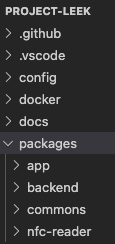
\includegraphics[width=3.8cm]{PackageStruktur.png}
  \caption{Orderstruktur}
  \label{fig:Orderstruktur}
\end{wrapfigure}
Die an das Projekt gesetzten Anforderungen machten die Erstellung mehrerer Applikationen notwendig. Neben einer Benutzeroberfläche, auf der die NFC-Tags
verwaltet werden können, musste die Steuerung des NFC-Readers und ein System zur Speicherung der Daten sowie zum Abspielen der Musik entwickelt werden.
Die dafür benötigten Anwendungen wurden als Microservices konzipiert und umgesetzt. Zur Verringerung des Aufwands der Konfiguration und Wartung wurden die einzelnen Microservices in einem Mono-Repository auf GitHub zusammengefasst.
Jeder Service wurde in einem Unterdner in \textit{packages} angelegt (vgl. Abbildung \ref{fig:Orderstruktur}). Der Ordner \textit{app} enthält die Benutzeroberfläche,
\textit{backed} die Datenbankschnittstelle sowie Logik zur Kommunikation mit dem Musik-Streaming-Anbieter und \textit{nfc-reader} die Applikation zum Steuern und auslesen des am Raspberry Pi angeschlossenen NFC-Readers.
Im Ordner commons befinden sich von allen Services gemeinsam genutzte Ressourcen (wie z. B. Modell-Klassen).
Neben den einzelnen Microservices wurden ebenfalls die Dokumentationsdateien wie Setup-Guide, Benutzerdokumentation und Projektbericht im Mono-Repo im Ordner \textit{docs} abgelegt.
Auch die für den Dienst \textit{Docker} benötigten Dateien fanden in dem gleichnamigen Ordner Platz. Die Konfigurationsdateien für \textit{ESLint} und den \textit{Typescript}-Compiler sind im Ordner \textit{config} zu finden.
Auf die Auflistung aller weiteren Dateien wird in diesem Bericht verzichtet. Eine genaue Aufstellung ist dem \textit{GitHub-Repository}\footnote{\url{https://github.com/project-leek/project-leek}} zu entnehmen.
Durch die Zusammenfassung in ein Mono-Repository waren die einzelnen Services für jeden Entwickler jederzeit einfach erreichbar, ohne die Notwendigkeit das Repository zu wechseln.



\subsection{Technologien und Hilfsmittel}
\colorbox{red}{TODO:}Vue, vscode, devops krams, etc
Entwickelt wird mit Visual Studio Code, da es eine einfache Nutzung des Linux-Subsystems ermöglicht. \footnote{https://code.visualstudio.com/docs/remote/wsl}.

\subsection{Projekt Management}
\colorbox{red}{ticket pool in github, alles zentral}

\subsection{Deployment Cycle}
\colorbox{red}{ziehe ticket > assigne dich selbst > draft PR > wenn fertig, setzte "undraft" > assigne 2 reviewer > merge master}

\section{Projekt Meilensteine}
\subsection{Meilenstein 1}
\colorbox{red}{TODO:}Kurze Einleitung, von wann bis wann ging
\subsubsection{Ziel}
\colorbox{red}{TODO:}was haben wir uns vorgenommen, was war das ziel, was wollten wir schaffen?
\subsubsection{Probleme}
\colorbox{red}{TODO:}welche prrobleme sind aufgetreten?

\subsubsection{Lösungen}
\colorbox{red}{TODO:}Welche Lösungen haben wir gefunden?

\subsubsection{Product Increment}
\colorbox{red}{TODO:}Was ist am Ende dabei rumgekommen?

\subsubsection{Retrospektive}
\colorbox{red}{TODO:}Was haben wir dabei gelernt? Neue Erkentnisse? Neue Sichtweisen?
Was lief gut, neu gelernt, was lief nicht so gut, was verbessern?
\begin{comment}{

Lief Gut
- Zusammenarbeit und Team Environment
- Meetings und Zusammenarbeit
- GitHub Workflow
- Anton!!!
- Richtig viel gelernt.
- Sau viel Zeit Einsatz von Anton, muss man mal wertschätzen.
- gruppenklima
- Die Kommunikation war klasse, genauso Teamwork.

Neu Gelernt
- Vue
- Feathers
- Tailwind
- CI
- undefined & null
- feathers
- vue
- Code / PR Review

Nicht so gut
- globale Probleme waren meh
- bei Problemen (nicht weitergekommen) nicht sofort bescheid sagen
- Wörtlicher Kundenwunsch wurde viel zu spät in dem sprint behandelt. Auch wenn hello wolrd cool war müssen wir vielleicht in dem nächsten sprint härter priorisieren.

Verbessern
- Aufgabenaufteilung
- Code reviews häufiger machen
- Aufgaben früher
- Teils lange Wartezeiten
- mehr den aktuellen stand kommunizieren
- Pünktlichkeit und rumorganisation der stand ups.
}

\subsection{Meilenstein 2}
\colorbox{red}{TODO:}Kurze Einleitung,  von wann bis wann ging}
\subsubsection{Ziel}
\colorbox{red}{TODO:}was haben wir uns vorgenommen, was war das ziel, was wollten wir schaffen?}
\subsubsection{Probleme}
\colorbox{red}{TODO:}welche prrobleme sind aufgetreten?}

\subsubsection{Lösungen}
\colorbox{red}{TODO:}Welche Lösungen haben wir gefunden?}

\subsubsection{Product Increment}
\colorbox{red}{TODO:}Was ist am Ende dabei rumgekommen?}

\subsubsection{Retrospektive}
\colorbox{red}{TODO:}Was haben wir dabei gelernt? Neue Erkentnisse? Neue Sichtweisen?
Was lief gut, neu gelernt, was lief nicht so gut, was verbessern?}
\colorbox{red}{TODO:}
  Gut
- Pair Programming
- (GitHub) workflow
- team arbeit
- Gegenseitige Hilfe
- Workflow lief besser

gelernt
- Viel Technisches (Feathers, Hooks, OAuth)
- manchmal weniger komplex denken und mehr an konkreten Problemen arbeiten
- Latex

nicht so gut
- abhängigkeiten von tickets (zumindest augenscheinlich, manchmal ist das gar nicht so der fall)
- Alles zu sehr gefühlt voneinander noch dependant, dass manche länger mal auf andere Sachen warten müssen

Verbessern
- Früher nachfragen
- probleme direkter ansprechen
- mehr pair-programming
- Presentation besser vorbereiten und vorher durchgehen
- in Daily: Cooolen Code vorstellen
- Definition-of-Done erstellen
- letzter Punkt, sollte sich aber von selber lösen
\end{comment}

\subsection{Meilenstein 3}
\colorbox{red}{TODO:}Kurze Einleitung,  von wann bis wann ging
\subsubsection{Ziel}
\colorbox{red}{TODO:}was haben wir uns vorgenommen, was war das ziel, was wollten wir schaffen?
\subsubsection{Probleme}
\colorbox{red}{TODO:}welche prrobleme sind aufgetreten?

\subsubsection{Lösungen}
\colorbox{red}{TODO:}Welche Lösungen haben wir gefunden?

\subsubsection{Product Increment}
\colorbox{red}{TODO:}Was ist am Ende dabei rumgekommen?

\subsubsection{Retrospektive}
\colorbox{red}{TODO:}Was haben wir dabei gelernt? Neue Erkentnisse? Neue Sichtweisen?
Was lief gut, neu gelernt, was lief nicht so gut, was verbessern?
\begin{comment}{
Lief Gut
- gemeinsames synchrones Arbeiten (gegen Ende)
- Teamreview
- ehrliches Miteinander
- Trotz Komplikationen und Probleme am Ende ein schönes Product Increment abgeliefert.
- Team Review hat gefühlt auch die Spannung gelöst und war sehr gut ehrlich zueinander zu sein.
- Pull Requests eindeutiger beschrieben ausgeführt (Mit Beispielen)
- Reviews schneller gemacht
- Feedback im Team
- Wichtige neue Features fertig gestellt (UI-components, Welcome Screen, Home Screen, Add-Tag Screen)
- Teamtreffen

Neu Gelernt
- stabiles Wissen mit vue (vor allem reactivity, events und components)
- Vue Parent/Child Kommunikation.
- Ein bisschen TailwindCSS.
- Neuer Vue Krams (inject & provide)
- Vue inject & provide
- Vue Prototypes
- Raspi comitup (hotspot zum WLan einrichten)


Nicht so gut
- scope des milestones: zu viele Sachen
- seeehr knappes sprintende
- Umplanung gegen Ende des Sprints
- Kommunikation und Absprache.
- Zeitmanagement.
- Fokus, was wir wirklich erledigen, was ist wichtig, was muss mindestens da sein und haben wir noch genug Zeit.
- Eingesetzte Zeit und Aufwand
- Wenig getestete Features
- Zu wenig Kommunikation zwischen den einzelnen Tickets bei Abhängigkeiten
- Meine Technik
- Zeit für Milestone / Sprint über Weihnachten & Neujahr zu lang

Verbessern
- besser abstimmmen was im Sprint gemacht werden soll
- nicht nur 'ja machen wir mal das hier alles'
- rechtzeitiger fragen bei Problemen
- Einen Tag vorher fertig mindestens
- reviews rechtzeitiger '^^
- Bessere Kommunikation und Absprache damit Ziele und Ansprüche klarer sind.
- Auch (inspiriert durch Julian) mehr "Gemeinsam lösen wir das Problem" Mindset anstelle "Wieso hast du das und das nicht gemacht?" Blameset.
- Insgesamt positiveres Mindset, denn wir schaffen ja doch schon viel.
- Zum vorletzten Daily die letzten Fixes ansprechen, dass am letzten Daily eigentlich nichts mehr ansteht.
- Fertig bis zum Vortag des nächsten Reviews
- Püntlicher zu Meetings erscheinen (Ich selbst)
- Kürzere Deadlines
- Ziele wiederholen in Meetings / klar festlegen: Was wird vom wem bis wann gemacht.
- Reviews schneller machen
- Aufgaben in kleinere Aufgaben teilen
- Zwischenstände zeigen lassen bei längeren Aufgaben
\end{comment}

\subsection{Meilenstein 4}
\colorbox{red}{TODO:}Kurze Einleitung, von, bis
\subsubsection{Ziel}
\colorbox{red}{TODO:}was haben wir uns vorgenommen, was war das ziel, was wollten wir schaffen?
\subsubsection{Probleme}
\colorbox{red}{TODO:}welche prrobleme sind aufgetreten?

\subsubsection{Lösungen}
\colorbox{red}{TODO:}Welche Lösungen haben wir gefunden?

\subsubsection{Erkenntnisse}
\colorbox{red}{Was haben wir dabei gelernt? Neue Erkentnisse? Neue Sichtweisen?}

\subsubsection{Product Increment}
\colorbox{red}{TODO:}Was ist am Ende dabei rumgekommen?

\subsubsection{Retrospektive}
\colorbox{red}{TODO:}Was haben wir dabei gelernt? Neue Erkentnisse? Neue Sichtweisen?
Was lief gut, neu gelernt, was lief nicht so gut, was verbessern?

\section{Code Walkthrough}
\colorbox{red}{TODO:}vielleicht interessante Code Snippets?

\section{Testing}
Das Team entschied sich zu Beginn der Produkt-Entwicklung dafür, Tests zur Verbesserung der Codequalität durchzuführen.
Quellcode Tests lassen sich in statische und dynamische Tests unterteilen.

\subsection{Statische Tests}
Im Allgemeinen untersuchen statische Tests nur Textdokumente und betrachten im Gegensatz zu dynamischen Tests nicht das Verhalten zur Laufzeit.
Dies ermöglicht eine häufige und kontinuierliche Nutzung von Tests dieser Art.
Zwei der prominenten Varianten statischer Tests, Linting und Reviews, wurden in diesem Projekt genutzt.

\subsubsection{Linting}
Beim Linting wurde der Code auf syntaktische Korrektheit geprüft.
Auch manche semantische (laufzeitunabhängige) Aspekte wurden untersucht.
So konnten kleinere Denkfehler und Flüchtigkeitsfehler, wie z. B. fehlende Kommata, schnell gefunden und behoben werden.
Hierfür wurde das Analyse-Werkzeug \textit{ESLint}\footnote{\raggedright\url{https://eslint.org/}} genutzt.
Für diese Werkzeug war zusätzlich auch eine Erweiterung\footnote{\raggedright\url{https://marketplace.visualstudio.com/items?itemName=dbaeumer.vscode-eslint}} für die Entwicklungsumgebung verfügbar.
Mit dieser konnten die Ergebnisse des Linting direkt im Code angezeigt werden.
Dies machte den Arbeitsprozess wesentlich zeiteffizienter.
Zusätzlich wurde auch die Erweiterung \textit{Vetur}\footnote{\raggedright\url{https://vuejs.github.io/vetur/}} genutzt.
Diese stellte die selben Funktionalitäten für den Vue-Framework spezifischen Code zur Verfügung.
\\
Darüber hinaus boten diese Erweiterungen auch Formatierungshilfen mit übertragbaren Konfigurationen.
Durch deren Nutzung konnte ein konsistenter Code-Stil innerhalb des Teams ermöglicht werden.
Dies legte den Grundstein für lesbaren Code und ermöglichte successive effizientes Arbeiten.

\subsubsection{Reviews}
Teil des Deployment Cycles waren auch Reviews der aktive Änderungen.
Bei diesen wurde der neue bzw. geänderte Quellcode von mindestens zwei anderen Teammitgliedern überprüft.
Untersucht wurden vor allem semantische Fehler, Lesbarkeit, Wartbarkeit und Vollständigkeit.
Hierfür gab es keinen formalen Plan, allerdings war die Review-Oberfläche von GitHub sehr hilfreich.
In dieser wurde eine Änderungsansicht (\textit{diff}) des zu überprüfenden Codes angezeigt.
So waren alle Teile des neuen Codes auf einen Blick einsehbar.
Darüber hinaus bot die Review-Oberfläche auch die Möglichkeit direkt im Code einzelne oder mehrere Zeilen zu kommentieren.
So konnten auch Änderungsvorschläge gemacht und direkt übernommen werden.
Dies sorgte für einen effizienten Review-Prozess.

\subsection{Dynamische Tests}
Als dynamische Tests wurden in diesem Projekt Anwendungsfall-basierte Tests genutzt.
Bei dieser Art von Test werden auf User-Stories aufbauende Testfälle herangezogen.
Diese Testfälle werden Schritt für Schritt \glqq durchgespielt\grqq.
Dabei wird überprüft, ob das tatsächliche Ergebnis dem erwartetem entspricht.
Die meisten Test  dieser Art wurden als Integrations-Tests durchgeführt.
Bei diesen wurde die Änderungen im Kontext der bestehenden Software getestet.
So konnte vor allem das Zusammenspiel von Frontend und NFC-reader mit dem Backend gut überprüft werden.
Aufgrund der Komplexität dieser Kontrollen wurden diese manuell durchgeführt und nicht automatisiert.
Diese Tests waren Teil des Deployment Cycles und wurden so in den meisten Fällen parallel zu den Reviews durchgeführt.
\\ \\
Ein gewisser Teil der anwendungsfallbasierten Test fand auf der Ebene von Code-Funktionen (\textit{Units}) statt.
Diese Unit-Tests wurden zur einfacheren Wiederholbarkeit automatisiert.
Dazu wurde das JavaScript-Test-Framework \textit{Jest}\footnote{\raggedright\url{https://jestjs.io/}} genutzt.
Dieses wurde gewählt, da sich Tests hiermit sehr intuitiv und ohne großen Lernaufwand schreiben ließen.
Auch diese Tests waren Teil des Deployment Cycles und wurden so bei jedem Pull-Request automatisch ausgeführt.



\section{Fazit}
\subsection{Probleme, Lösungen, Erkenntnisse}
\colorbox{red}{TODO: Finde TITEL:} Fazit oder nur Erkenntnisse oder oder?
\colorbox{red}{Besseres Intro zum Kapitel?}
Das Projekt Informatik gab einen realistischen Einblick in die Arbeitswelt. Das Team musste sich klassischen Alltagsproblemen stellen, Lösungswege finden und wichtige Erkenntnisse für die Zukunft daraus ziehen.
Auch Coding-Entwurfsmuster und -Konventionen wurden neu erlernt und praktisch angewandt.

\subsubsection{Einarbeitung in neue Technologien}
Zu Beginn des Projektes bestand eine größere Differenz, inwieweit die einzelnen Teammitglieder mit den jeweiligen Technologien vertraut waren.
Insbesondere die Projektstruktur bereitete aufgrund der höheren Komplexität eine größere Einstiegshürde für viele Entwickler.
Dies lag darin begründet, dass die vielen automatisch generierten Dateien und Ordner anfangs zu Unübersichtlichkeit führten.
Mit zunehmender Entwicklungszeit und durch die Arbeit an den Teilkomponenten des Mono-Repositorys gewannen die Entwickler jedoch schnell mehr Überblick über die Struktur.
Über die Entwicklungszeit wurden aber die neuen Technologien vertieft und verinnerlicht.
Das Team lernte wie Frameworks und Libraries  z. B. Vue, Tailwind und Feathers sinnvoll und hilfreich eingesetzt werden können.

\subsubsection{Versionskontrolle und Deployment Cycle}
Zwar wurde den Studierenden im Studium der Vorteil von Versionskontrollsystemen wie Git vermittelt, doch fand sich im Studium selten ein praktisches Anwendungszenario, dass Git über die Hauptfunktion der Versionierung hinaus sinnvoll genutzt hat.
Dieses Projekt bot erstmals eine sinnvolle Anwendung von \textit{git} uns zeigte, wie in größeren Projekten oder in der Industrie auch mit Pull Requests und Code Reviews zu arbeiten.
Diese Methoden führten zu folgenden maßgebliche Verbesserungen:
Durch die erforderten zwei Code Reviews pro Pull Request wurde Fehler im Code häufiger entdeckt und eine höhere Codequalität wurde sichergestellt.
Als positiver Nebeneffekt konnten die Reviewer außerdem während des Prozesses neue Funktionen und Codemuster erlernen, zu denen sie bei Bedarf (per Kommentar) Fragen stellen konnten.
Die Gewöhnung an diesen Deployment Cycle brauchte eine gewisse Zeit, fand aber von Sprint zu Sprint immer mehr Wertschätzung im Team.
Sich an diesen Deployment Cycle zu gewöhnen brauchte eine gewisse Zeit, aber fand von Sprint zu Sprint immer mehr Wertschätzung im Team.

\subsubsection{Automatisierte Tests und Deployment}
Jeder Pull Request durchlief außerdem mehrere automatisierte Tests - sogenannte \textit{Actions}.
Diese prüften den Quellcode anhand fest eingestellter Testparameter.
Durch diese Tests wurde dem Team viel manuelle Arbeit abgenommen und die Fehlerquelle Mensch minimiert.
Neue Änderungen im Master wurden automatisch auf Github.io veröffentlicht, als auch wurden die \textit{LaTeX} Dateien als PDF im eigenen Dokumente Branch gebaut.
Für Pull Requests wurde auch die jeweilige Version gebaut und auf einer \colorbox{yellow}{temporären} Webseite veröffentlicht.
Dank dieser Automatisierungen konnte sich das Team mehr auf das Weiterentwickeln des Projektes konzentrieren.

\subsubsection{Regelmäßige Standups und Retrospektiven}
Durch die regelmäßigen Standups entstand ein Ort für gegenseitigen Austausch von Problemen und Informationen über Fortschritt und neue Funktionen.
So wurde verhindert, dass Probleme untergingen, neues Wissen wurde schneller verbreitet und die gesamte Teamproduktivität verbessert.
Das bei den Retrospektiven entstandene Feedback erwies sich als sehr wichtig für das Teamklima.
Auch die hierbei angesprochenen Probleme und Verbesserungsvorschläge wurden vom Team als sehr wertvoll für die nächsten Sprints erkannt und entsprechend adaptiert.

\subsubsection{Kommunikation und Eigeninitiative}
Die Standups hatten auch den Effekt, dass das Team sich anfangs zu sehr auf diesen Kommunikationsweg verließ, wodurch Probleme und wichtige Kommunikation bei Abhängigkeit zwischen Tickets teilweise zu selten stattfanden.
Tickets wurden anfangs sehr groß gefasst.
Dadurch entstand der Eindruck, dass diese Tickets sehr komplex und schwierig wären.
Hier fehlte anfangs die Eigeninitiative, sich aktiv Hilfe zu holen, um diese zu bearbeiten oder die Tickets in kleinere Tickets aufzuteilen.
Hierbei halfen einerseits die Retrospektiven, in denen dieses Problem angesprochen wurde, sowie vor allem die teaminternen Evaluationen.

\subsubsection{Planung, Zielsetzung und Einschätzung}
Das größte Problem während des Projektes war, dass gegen Ende eines Sprints geplante Tickets teilweise nicht fertiggestellt wurden.
Häufig konnten nicht alle Tickets genügend auf Fehler getestet werden und wurden entweder in den nächsten Sprint verschoben oder mit kleineren Bugs in den Master Branch gemerged.
Hier wurden oftmals Überstunden geleistet und das Team hat hier besonders gelernt, wie wichtig Planung der Tickets sowie das Einschätzen der eigenen Leistung zur Bewältigung verschiedenster Probleme ist.
So hat das Team sich auch vorgenommen, mindestens zwei Tage vor einem Sprintende alle für den Sprint benötigten Tickets fertiggestellt zu haben.
Dadurch sollte genügend Zeit geschaffen werden, um Tickets auf Fehlerfreiheit zu testen und konfliktfrei in den Master Branch mergen zu können.
Auch wenn die Lösung dieses Problem hätte effizienter behandelt werden können, war diese Methode angesichts der knappen Projektlaufzeit die effektivste.

\section{Technische Diagramme}
\colorbox{red}{TODO:}ER Diagramme, UML, solcher krams

\newpage
\section{Anhang}
\colorbox{red}{BEISPIEL, DELETE THIS} Buchreferenz \cite{Literaturbeispiel:tom} oder Seitenref \cite{google}
\printbibliography
\end{document}
